% ================================================================
% Drop-in replacement for the visualized Inner Comparison section.
% Table 2 and Table 3 remain in the existing experiment source.
% Required package in the parent paper: \usepackage{graphicx}
% Generated figures live under: figure/experiment_picture/
% ================================================================

\subsection{Inner Comparison}
\label{sec:inner_comparison}

The cross-method and matched-fit results establish external effectiveness and
isolate the contribution of teacher-conditioned deflection. We next hold the
backbone, rendered inputs, pseudo labels, and evaluation protocol fixed, and
visualize three narrower claims: whether the native numeric channel remains
limiting under stronger prompting controls; whether the gain concentrates in
teacher--human disagreement regimes; and whether the learned context-attention
pattern is functionally responsible for the score. Exact numerical values are
retained in the appendix tables.


\subsubsection{Native Scoring Channel}
\label{sec:native_channel}

All prompting controls use the same frozen backbone, multimodal input, and
evaluation rubric. They differ only in how the native language channel is
elicited. Figure~\ref{fig:native_accuracy_resolution} separates human-aligned
performance from score resolution rather than compressing both into one
multi-axis plot.

\begin{figure*}[t]
    \centering
    \begin{minipage}[t]{0.49\textwidth}
        \centering
        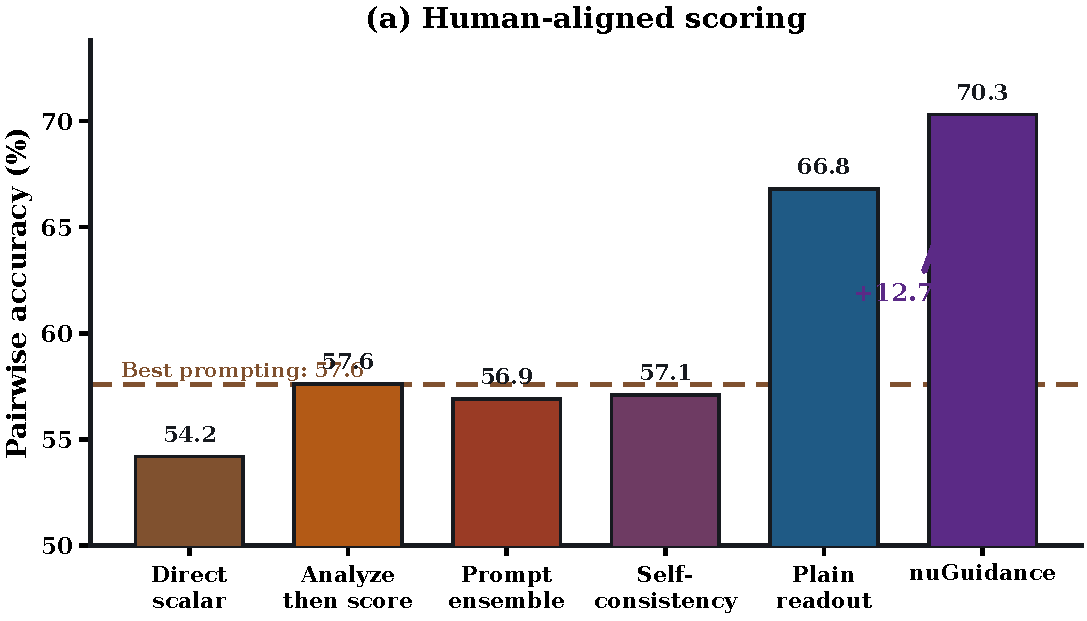
\includegraphics[width=\linewidth]
        {figure/experiment_picture/fig4a_pairwise_accuracy.pdf}
    \end{minipage}
    \hfill
    \begin{minipage}[t]{0.49\textwidth}
        \centering
        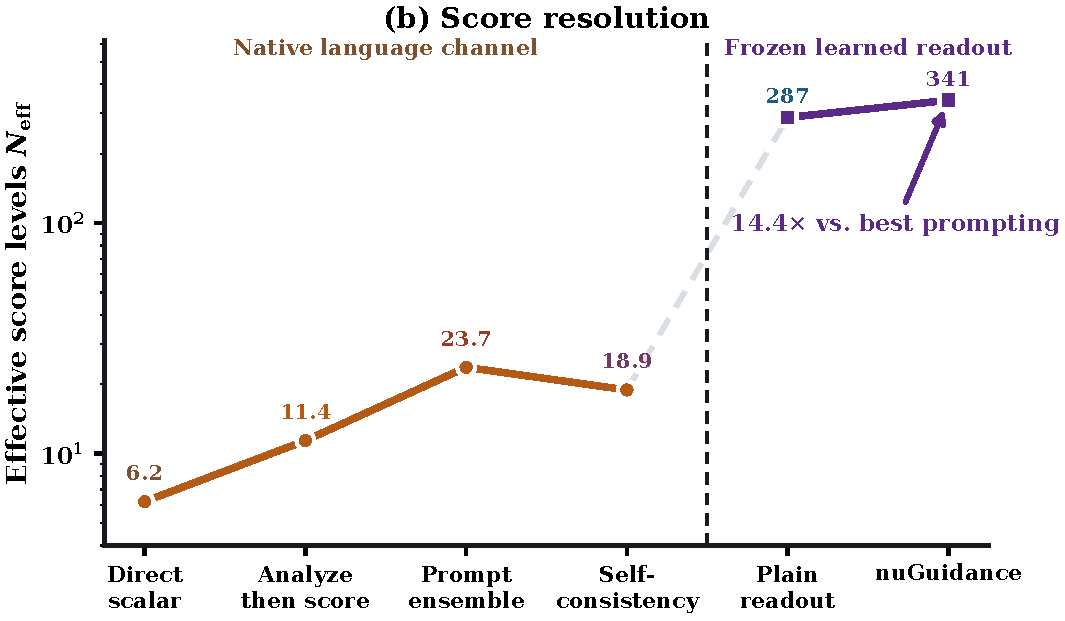
\includegraphics[width=\linewidth]
        {figure/experiment_picture/fig4b_effective_levels.pdf}
    \end{minipage}
    \caption{
        \textbf{Native textual scoring versus frozen learned readout.}
        Left: WOD-E2E pairwise accuracy. Right: effective score resolution
        $N_{\mathrm{eff}}$ on a logarithmic scale. Stronger prompting,
        paraphrase ensembling, and repeated sampling remain below the learned
        readouts. \methodname{} reaches 70.3\% pairwise accuracy and 341
        effective score levels, compared with 57.6\% and 23.7 for the strongest
        prompting controls.
    }
    \label{fig:native_accuracy_resolution}
\end{figure*}

Figure~\ref{fig:native_accuracy_resolution} shows a clean separation between
prompt engineering and learned readout. Analyze-then-score is the strongest
native-channel control at 57.6\% pairwise accuracy, but the plain frozen
readout reaches 66.8\%, and \methodname{} reaches 70.3\%. The same separation
appears in score resolution: \methodname{} exposes 341 effective levels,
$14.4\times$ the 23.7 levels obtained by the strongest prompting control.
Thus, better prompting improves neither human alignment nor score granularity
enough to close the readout gap.

\begin{figure*}[t]
    \centering
    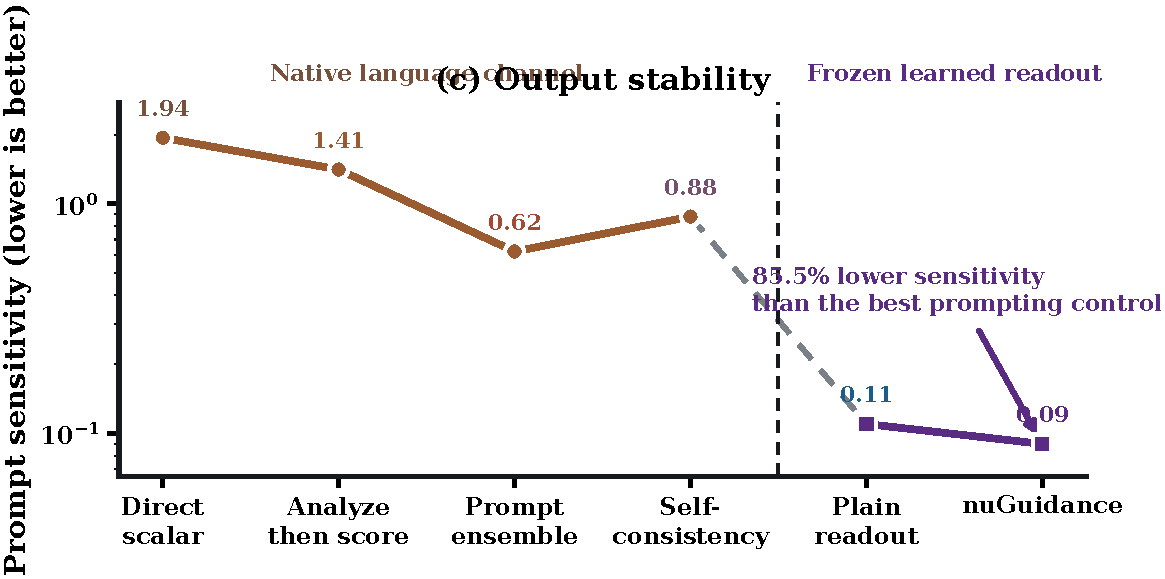
\includegraphics[width=0.70\textwidth]
    {figure/experiment_picture/fig4c_prompt_sensitivity.pdf}
    \caption{
        \textbf{Prompt sensitivity of the native channel.}
        The first four points are textual scoring controls; the final two are
        frozen learned readouts. Lower is better. The best prompting control
        remains at 0.62 sensitivity, whereas \methodname{} reaches 0.09, an
        85.5\% reduction.
    }
    \label{fig:native_prompt_sensitivity}
\end{figure*}

The stability result in Fig.~\ref{fig:native_prompt_sensitivity} rules out the
simpler explanation that the direct-prompt baseline merely used one brittle
wording. Ensembling reduces sensitivity, but it does not recover the accuracy
or score resolution of the learned readout. Together, the three plots support
a channel bottleneck: the frozen representation can support substantially
better scoring than the native textual number interface reports.


\subsubsection{Semantic Disagreement Regimes}
\label{sec:disagreement_regimes}

Overall MAE can conceal whether an evaluator succeeds on the cases that
motivate semantic scoring. We therefore partition WOD-E2E using the fixed
Scheme-B teacher score, public rule outputs, and existing human ratings, with
no model-dependent manual case selection.

\begin{figure*}[t]
    \centering
    \begin{minipage}[t]{0.52\textwidth}
        \centering
        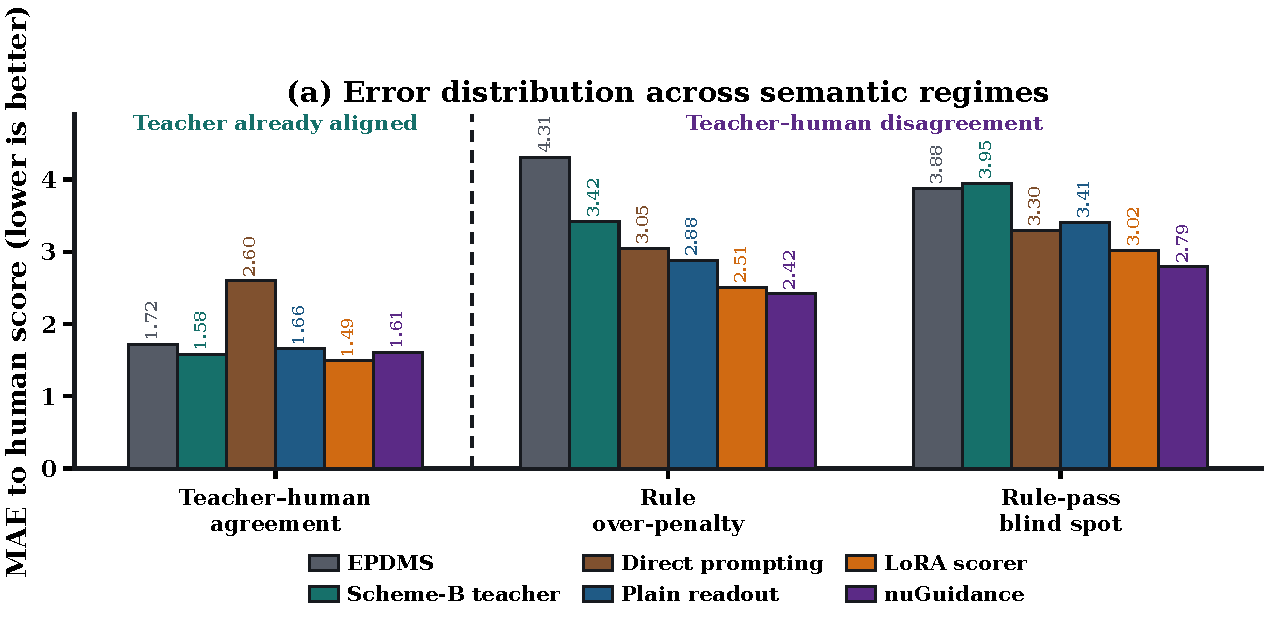
\includegraphics[width=\linewidth]
        {figure/experiment_picture/fig5a_regime_grouped_bars.pdf}
    \end{minipage}
    \hfill
    \begin{minipage}[t]{0.46\textwidth}
        \centering
        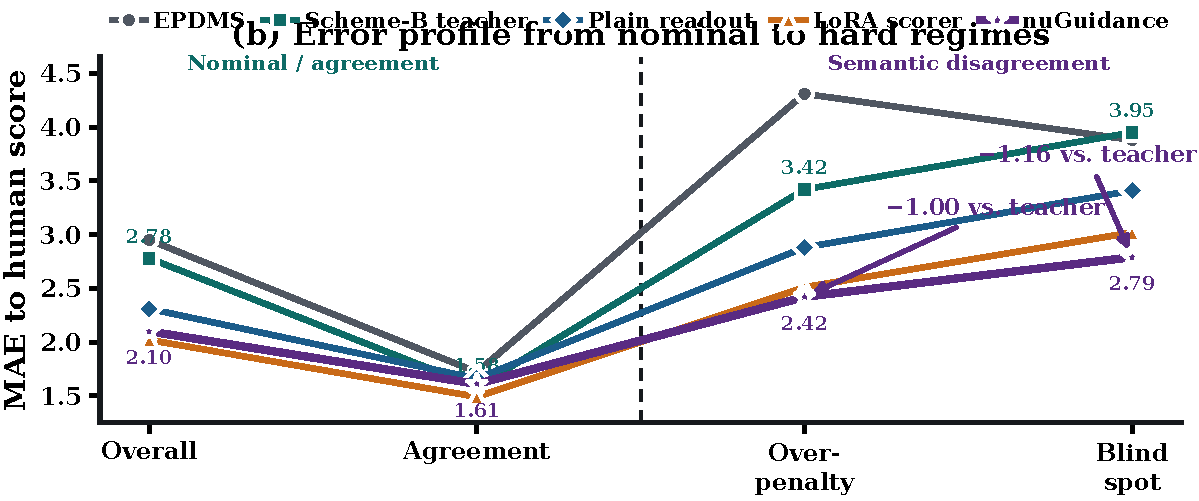
\includegraphics[width=\linewidth]
        {figure/experiment_picture/fig5b_error_profile_line.pdf}
    \end{minipage}
    \caption{
        \textbf{Human-alignment error across semantic regimes.}
        Left: grouped MAE comparison on teacher--human agreement,
        rule over-penalty, and rule-pass blind-spot subsets. Right: the same
        methods traced from overall performance to the increasingly difficult
        semantic regimes. \methodname{} reduces teacher MAE by 1.00 point on
        rule over-penalty cases and by 1.16 points on rule-pass blind spots.
    }
    \label{fig:semantic_regime_results}
\end{figure*}

The regime breakdown in Fig.~\ref{fig:semantic_regime_results} distinguishes
semantic correction from ordinary teacher fitting. On the agreement subset,
\methodname{} is close to the teacher (1.61 versus 1.58 MAE), so its overall
gain is not obtained by perturbing already-correct cases. The advantage
appears where context is necessary: over-penalty MAE falls from 3.42 for the
teacher to 2.42, and rule-pass blind-spot MAE falls from 3.95 to 2.79. The
plain readout remains at 2.88 and 3.41, respectively, showing that the hard-case
benefit is not explained by pseudo-score distillation alone.

\begin{figure*}[t]
    \centering
    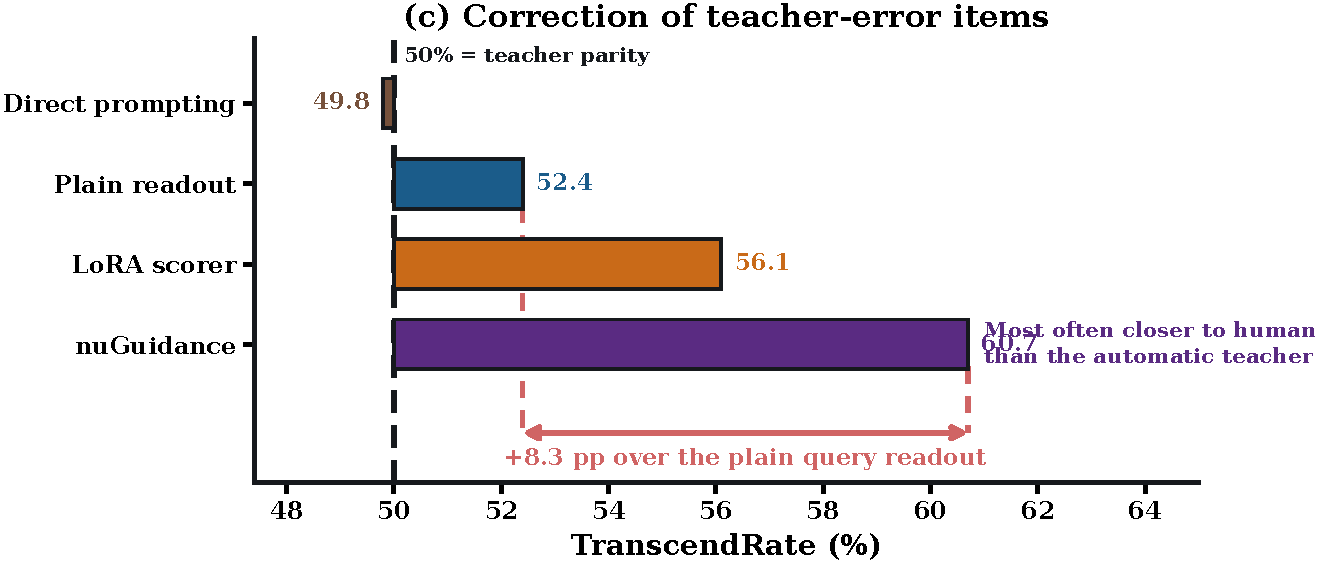
\includegraphics[width=0.62\textwidth]
    {figure/experiment_picture/fig5c_transcend_rate.pdf}
    \caption{
        \textbf{Correction of teacher-error items.}
        TranscendRate is the proportion of disagreement items on which the
        student is closer to the existing human score than the Scheme-B
        teacher. The dashed 50\% line is the teacher-parity reference.
        \methodname{} reaches 60.7\%, compared with 52.4\% for the plain
        readout and 56.1\% for LoRA.
    }
    \label{fig:semantic_transcend_rate}
\end{figure*}

Figure~\ref{fig:semantic_transcend_rate} provides the direct teacher-inheritance
test. \methodname{} improves TranscendRate by 8.3 percentage points over the
plain readout and by 4.6 points over LoRA. This result supports, but does not
assume, weak-to-strong behavior: the student more often moves toward human
judgment on the teacher's identifiable failure regime. If this pattern does
not survive confidence intervals or the locked-test protocol, the conclusion
must be narrowed to faithful frozen pseudo-score distillation.


\subsubsection{Causal Readout Interventions}
\label{sec:causal_interventions}

We intervene on the exact context-attention branch used by the filtering
criterion. One trained \methodname{} checkpoint and scalar head are held fixed,
and no intervention is followed by retraining. Figure~\ref{fig:causal_drops}
reports changes relative to the unchanged readout, which is the relevant
paired causal comparison.

\begin{figure*}[t]
    \centering
    \begin{minipage}[t]{0.49\textwidth}
        \centering
        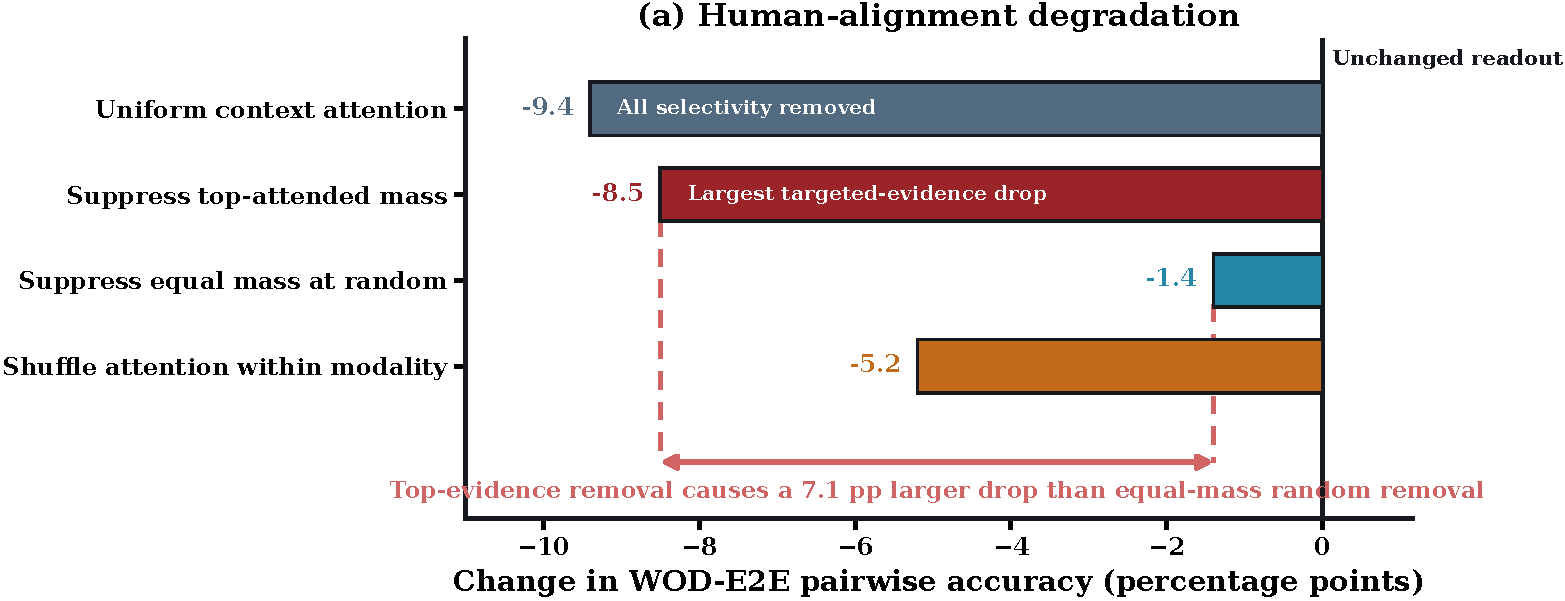
\includegraphics[width=\linewidth]
        {figure/experiment_picture/fig6a_delta_pairwise_accuracy.pdf}
    \end{minipage}
    \hfill
    \begin{minipage}[t]{0.49\textwidth}
        \centering
        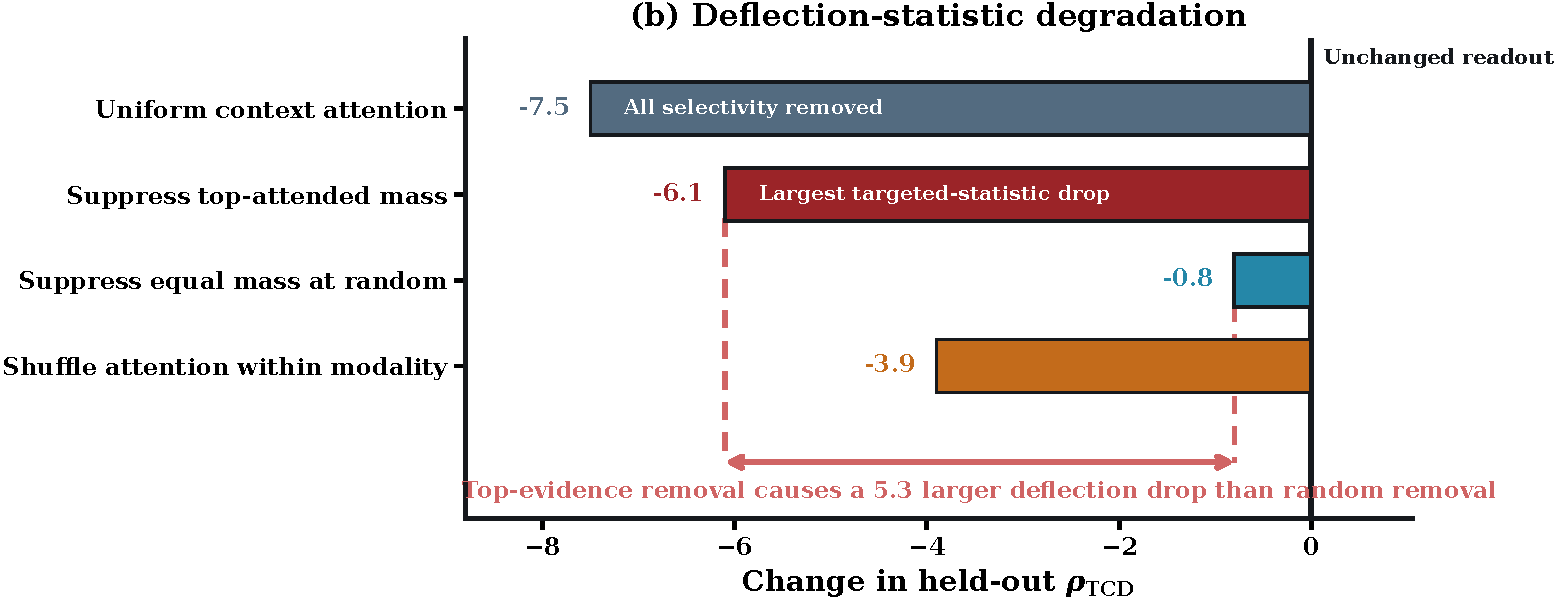
\includegraphics[width=\linewidth]
        {figure/experiment_picture/fig6b_delta_rho_tcd.pdf}
    \end{minipage}
    \caption{
        \textbf{Causal interventions on the learned attention readout.}
        Left: change in WOD-E2E pairwise accuracy. Right: change in held-out
        $\rho_{\mathrm{TCD}}$. Suppressing top-attended context mass costs
        8.5 accuracy points, compared with 1.4 points for equal-mass random
        suppression; the corresponding deflection drops are 6.1 and 0.8.
        Every bar is measured relative to the same unchanged checkpoint.
    }
    \label{fig:causal_drops}
\end{figure*}

The intervention pattern is consistent across the external metric and the
internal statistic. Uniform attention causes the largest accuracy decline
($-9.4$ points), top-attended suppression causes an $-8.5$-point decline, and
within-modality shuffling causes an intermediate $-5.2$-point decline. Equal
attention mass removed at random costs only $-1.4$ points. The decisive
contrast is therefore 7.1 percentage points between top-attended and random
suppression, accompanied by a 5.3-point difference in the deflection drop.
Because the checkpoint and scalar head never change, this comparison supports
a functional role for the learned context-attention pattern rather than a
post-hoc visualization of an otherwise head-dominated scorer.
